% Notes:
% shell escape must be enabled
\documentclass[12pt, oneside]{report}

%Debugging packages and commands:
%\usepackage{showframe}
\overfullrule=10pt

% Modular Compilation
\usepackage{subfiles}
\providecommand{\main}{.}

% LETU Thesis Formatting
\usepackage{\main/letuThesis}
\usepackage[crop=pdfcrop]{pstool}
\usepackage{standalone} % for inputting tikz pictures

%\newcommand{\cftdot}{\ast}
%\newcommand{\cftdotsep}{2}
%% Change parameters for the LOF and LOT
%\makeatletter
%\renewcommand\@pnumwidth{1.55em} % Width for the page number to be typeset, default 1.55em
%\renewcommand\@tocrmarg{2em} % Margin between right margin and end of leader lines, default 2.55em
%\renewcommand\@dotsep{.5} % Separation between leader line dots, units=?
%
%\usepackage{tocloft}

%
%\makeatletter
%% Place the label in a \rlap to make chapters labels greater than 10 line up with same spacing
%\titlecontents{chapter}[0in]{
%    \pretolerance=1000\tolerance=1000\emergencystretch=1em
%    \singlespacing\hangindent=1em
%    }
%  {\contentspush{%
%      \MakeUppercase\@tocChapterName~\rlap{\thecontentslabel:}\hphantom{0:}}\quad
%    \MakeUppercase
%  }%
%  {\MakeUppercase}%
%  {\leaderStyle\contentspage}
%\makeatother
%
%\titlecontents{figure}[0in]%
%  {\singlespacing}{\contentspush{\rlap{\thecontentslabel}\hspace{2.5em}}}{}% 2.5em space between left margin and caption label text
%  {\leaderStyle\contentspage}
%
%\makeatother

%% Remove the extra space from between chapters in the lof/lot: https://tex.stackexchange.com/questions/121879/remove-spacing-between-per-chapter-figures-in-lof
%% Would be nice to place in an option...
%\usepackage{etoolbox}% http://ctan.org/pkg/etoolbox
%\makeatletter
%% \patchcmd{<cmd>}{<search>}{<replace>}{<succes>}{<failure>}
%\patchcmd{\@chapter}{\addtocontents{lof}{\protect\addvspace{10\p@}}}{}{}{}
%\patchcmd{\@chapter}{\addtocontents{lot}{\protect\addvspace{10\p@}}}{}{}{}
%\makeatother

%\usepackage{hyperref}
%%	\usepackage[linktocpage=true]{hyperref}
% above needs \phantomsection before calls to \addcontentsline


% External Packages
\usepackage{lipsum}

% Preamble Information
%\title{Real-Time \\ Model Predictive Control}
%\author{Jeremy Goossen}
%\committee{
%	Dr. G. Nathan Green, PhD \\ 
%	Dr. Joonwan Kim, PhD \\ 
%	Dr. Marian Iordache, PhD \\ 
%	Prof. Andrew Davis}
%\university{LeTourneau Univeristy}
%\school{School of Engineering and Engineering Technology}
%\discipline{Electrical Engineering}
%\titlepageauthor{J. Goossen}

\usepackage{graphicx}
\graphicspath{ {\main/figures/} }
\usepackage[hidelinks]{hyperref}
\begin{document}

\frontmatter

\maketitle
\makesignatures
\makecopyright

\unpacklipsum[1-3]
\makeabstract{\lipsumexp}

\makeacknowledgments{\lipsum[4-5]\par
I'd like to acknowledge everyone who made this possible. Thanks!\par}

\tableofcontents

%\clearpage
%\addcontentsline{toc}{chapter}{List of Tables}
%\chapter*{List of Tables}
\listoftables

%\clearpage
%\addcontentsline{toc}{chapter}{List of Figures}
%%\addtocontents{lof}{~\hfill Page\par}
\listoffigures





\mainmatter % Switch to Arabic numbering

\chapter{Introduction}
\lipsum[1]
%\section{Suspendisse vitae elit. Aliquam arcu neque, ornare in, ullamcorper quis, commodo eu, libero.} % \lipsum[10][1-2]
\section{\lipsum[150][1-3]}
\lipsum[3]%
\footnote{This is simply the ubiquitous ``Lorem Ipsum'' placeholder text for typesetting. This is a long footnote, and extends to more than just a single line.}

\begin{figure}[h]
  \centering
  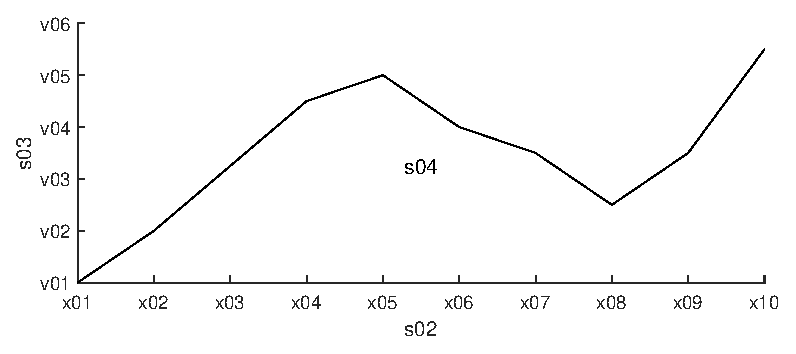
\includegraphics[width=.7\textwidth]{pictures/placeholder}
  \caption{The caption of the figure}
  \label{fig:BlockDiagram1}
\end{figure}
  
\begin{figure}[h]
  \centering
  \psfragfig[width=.99\textwidth]{figures/plots/placeholder}{}
  \caption{The caption of the figure which is much longer than the other captions, since it should flow to the next line every time}
  \label{fig:BlockDiagram2}
\end{figure}

\begin{figure}[h]
  \centering
  \includestandalone[mode=buildnew]{figures/diagrams/placeholder}
  \caption{The caption of the figure}
  \label{fig:BlockDiagram3}
\end{figure}

\begin{figure}[h]
  \centering
  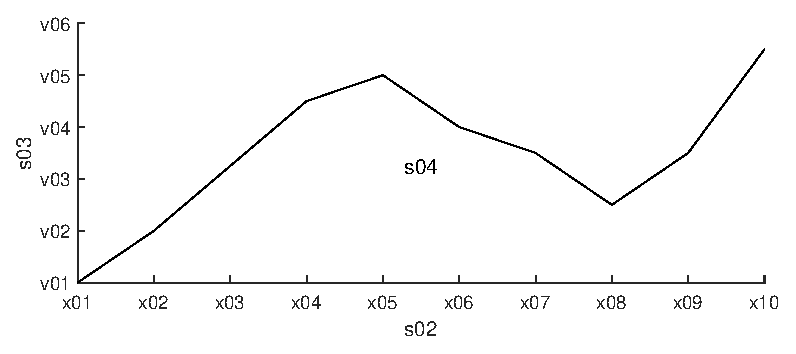
\includegraphics[width=0.5\textwidth]{pictures/placeholder}
  \caption{The caption of the figure}
  \label{fig:BlockDiagram4}
\end{figure}

\begin{figure}[h]
  \centering
  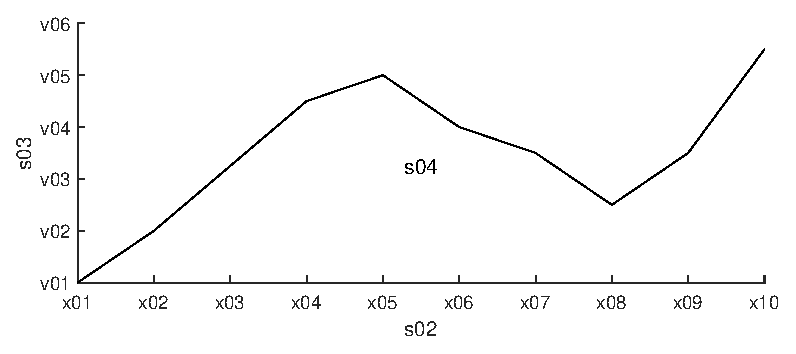
\includegraphics[width=0.5\textwidth]{pictures/placeholder}
  \caption{The caption of the figure}
  \label{fig:BlockDiagram4}
\end{figure}

\begin{figure}[h]
  \centering
  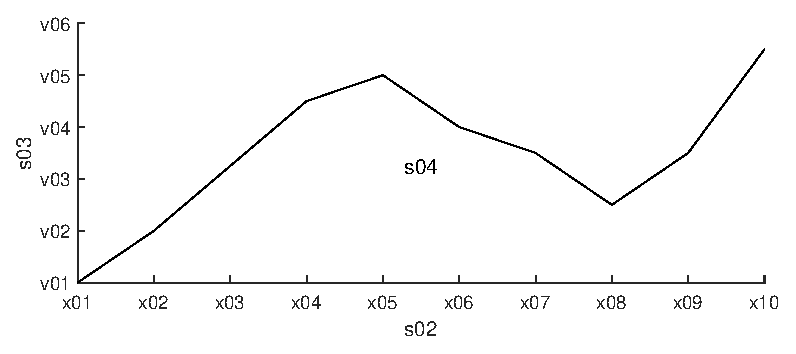
\includegraphics[width=0.5\textwidth]{pictures/placeholder}
  \caption{The caption of the figure}
  \label{fig:BlockDiagram4}
\end{figure}

\begin{figure}[h]
  \centering
  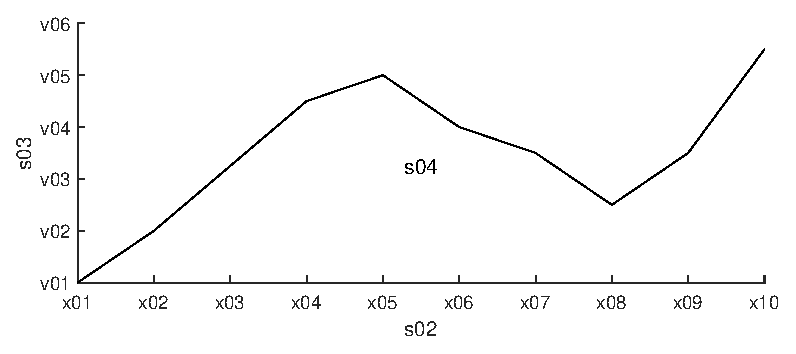
\includegraphics[width=0.5\textwidth]{pictures/placeholder}
  \caption{The caption of the figure}
  \label{fig:BlockDiagram4}
\end{figure}

\begin{figure}[h]
  \centering
  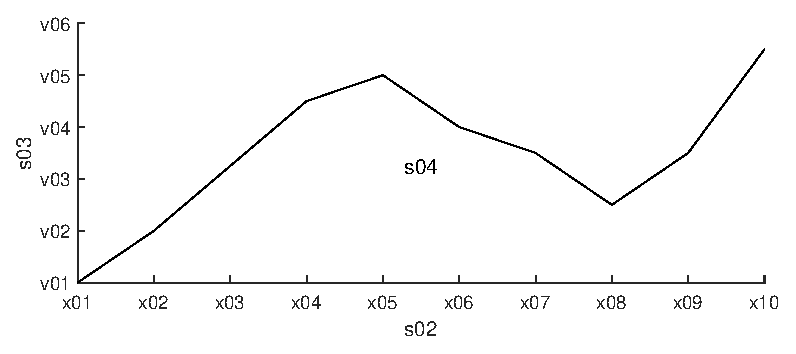
\includegraphics[width=0.5\textwidth]{pictures/placeholder}
  \caption{The caption of the figure}
  \label{fig:BlockDiagram4}
\end{figure}

\begin{figure}[h]
  \centering
  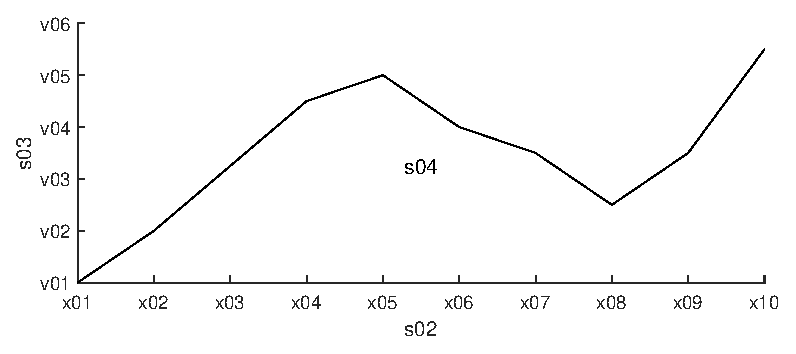
\includegraphics[width=0.5\textwidth]{pictures/placeholder}
  \caption{The caption of the figure}
  \label{fig:BlockDiagram4}
\end{figure}

\begin{figure}[h]
  \centering
  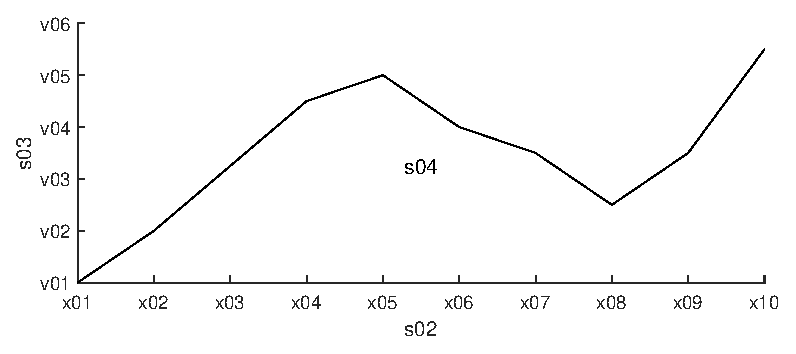
\includegraphics[width=0.5\textwidth]{pictures/placeholder}
  \caption{The caption of the figure}
  \label{fig:BlockDiagram4}
\end{figure}

\begin{figure}[h]
  \centering
  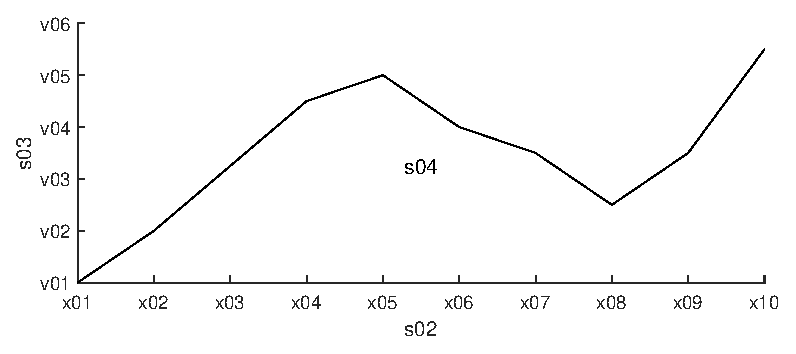
\includegraphics[width=0.5\textwidth]{pictures/placeholder}
  \caption{The caption of the figure}
  \label{fig:BlockDiagram4}
\end{figure}


%This paragraph references Figure \ref{fig:BlockDiagram1}, and should be clickable.

\lipsum[4]
\footnote{Another paragraph from the same source.}\footnote{And something else I remembered that merits its own footnote.}

\subsection{Subsection Title}
\lipsum[5]

\subsubsection{Sub-subsection}
\lipsum[6-7]
\subsubsection{Another Sub-subsection}
\lipsum[8-9]\footnote{This footnote is on a new page and is numbered starting from the beginning}

\section{\lipsum[150][4]}

\subsection{\lipsum[150][8]}
\lipsum[10]

\unpacklipsum[150][5]
\chapter{\lipsumexp}

\section{\lipsum[150][6]}
\lipsum[5-6]

\section{\lipsum[150][7]}
\lipsum[7]

\chapter{One}
\chapter{Another}
\chapter{Another}
\chapter{Another}
\chapter{Another}
\begin{figure}[h]
  \centering
  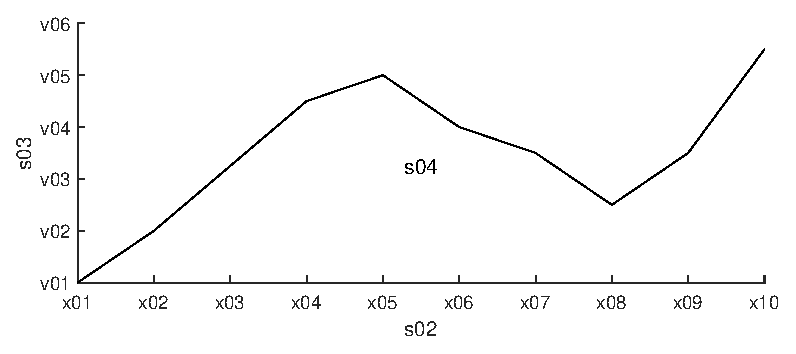
\includegraphics[width=0.5\textwidth]{pictures/placeholder}
  \caption{The caption of the figure}
  \label{fig:BlockDiagram4}
\end{figure}
\chapter{Another}
\chapter{Another}
\chapter{Another}
\chapter{Another}
\chapter{Another}
\chapter{Another}
\chapter{Another}
\chapter{Another}



\backmatter

\bibliographystyle{ieeetr}
\bibliography{\main/references/references}


\begin{appendices}

\unpacklipsum[141][1-3]
\chapter{\lipsumexp}
\lipsum[140][4]

\begin{figure}[h]
  \centering
  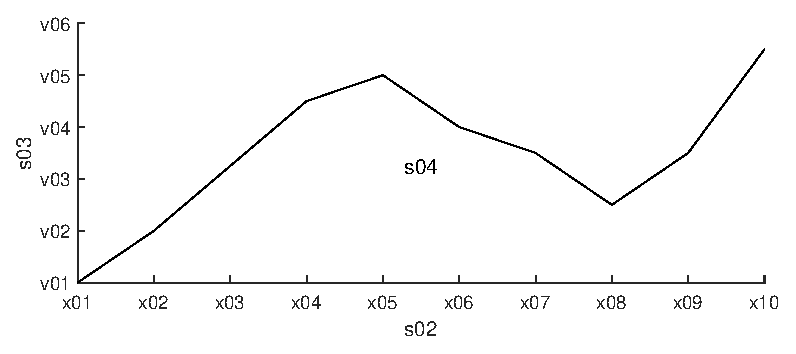
\includegraphics[width=0.5\textwidth]{pictures/placeholder}
  \caption{The caption of the figure}
  \label{fig:BlockDiagram4}
\end{figure}

\section{\lipsum[140][3]}
\lipsum[8-9]

\section{\lipsum[140][5]}
\lipsum[10]

\unpacklipsum[140][6]
\chapter{\lipsumexp}
\lipsum[11] \cite{einstein, latexcompanion, knuthwebsite}


\end{appendices}






\end{document}